\documentclass[11pt,a4paper]{article}

% Packages
\usepackage[utf8]{inputenc} % Encoding
\usepackage[T1]{fontenc}   % Font encoding
\usepackage{amsmath,amssymb,amsfonts} % Math packages
\usepackage{graphicx}      % For including graphics
\usepackage{hyperref}      % For hyperlinks
\usepackage{geometry}      % For page layout
\usepackage{float}         % For better float placement
\usepackage{enumitem}      % For custom lists
\usepackage{caption}       % For captions
\usepackage{subcaption}    % For subfigures
\usepackage{xcolor}        % For colored text
\usepackage{listings}
\usepackage{csvsimple}  % Package for handling CSV files

\lstset{
  basicstyle=\ttfamily\small,  % Use small monospaced font
  keywordstyle=\color{blue},  % Set color for keywords
  commentstyle=\color{green},  % Set color for comments
  stringstyle=\color{red},  % Set color for strings
  breaklines=true,  % Enable line breaking for long lines
  frame=single,  % Add a frame around the code
  showstringspaces=false  % Don't show spaces in strings
}
% Geometry settings
\geometry{
  a4paper,
  left=1in,
  right=1in,
  top=1in,
  bottom=1in
}

% Custom commands

% Title and Author
\title{Benchmarking CUDA Gaussian Kernel}
\author{Jacob DeRosa}
\date{\today}

\begin{document}

% Title Page
\maketitle
\tableofcontents
\newpage

% Sections
\section{Code Analysis}

\subsection{Implementation of Gaussian Kernel Caller/Setup}
\begin{lstlisting}
void gaussian_kde(int n, float h, const std::vector<float>& x, std::vector<float>& y) {

    cudaDeviceProp device_prop;
    cudaGetDeviceProperties(&device_prop, 0);

    int threadsPerBlock = int(h);

    h = 0.01;

    int xblocks = (n + threadsPerBlock - 1)/ threadsPerBlock;
   
    float *d_x, *d_y;

    cudaMalloc(&d_x, sizeof(float)*n);
    cudaMemcpy(d_x, x.data(), n*sizeof(float), cudaMemcpyHostToDevice);

    cudaMalloc(&d_y, sizeof(float)*n);
    
    float k = 1/(n*h);
    
    cudaDeviceSynchronize();    

    cudaError_t err = cudaGetLastError();
    if (err != cudaSuccess) {
        std::cerr << "CUDA error: " << cudaGetErrorString(err) << std::endl;
    }

    kde_kernel<<<xblocks, threadsPerBlock, threadsPerBlock*sizeof(float)>>>(d_x, d_y, n, h, k);

    cudaDeviceSynchronize();

    err = cudaGetLastError();
    if (err != cudaSuccess) {
        std::cerr << "CUDA error: " << cudaGetErrorString(err) << std::endl;
    }

    cudaMemcpy(y.data(), d_y, n * sizeof(float), cudaMemcpyDeviceToHost);

    cudaFree(d_x);
    cudaFree(d_y);

} // gaussian_kde
\end{lstlisting}
Here I am allocating memory for the device and managing the cuda kernel. First I divided the input by the $threadsPerBlock$ to determine the number of blocks.
Next I allocated memory for the input and output arrays $d\_x$ and $d\_y$ on the device. I calculated the bandwidth constant outside of the kernel.
Then I initialized the cuda kernel and copy the results from $d\_y$ back to host memory. This configuration assumes that the number of threads being spawned is less than the amount of active cuda threads the SM's can handle before exhausting their register and shared memory allocation.
It introduces a ceiling to the scaling capabilities of a single device.

\subsection{Implementation of Density Estimator CUDA kernel}
\begin{lstlisting}
__device__ float K(float x)
{
    return (1/(sqrtf(2*M_PI)))*expf(-(x*x)/2);
}

__global__ void kde_kernel(const float *x, float *y, int n, int h, float k)
{
    int bx = blockIdx.x;
    int idx = blockDim.x * bx + threadIdx.x;

    if (idx < n)
    {
        float xi = x[idx];

        for (int j = 0; j < n; j++)
        {
            int xj = x[j];
            y[idx] += K((xi - xj) / h);
        }
    }
}
\end{lstlisting}
In The $K$ (kernel) function I am using $sqrtf$ and $expf$ instead of their std::* counterparts becuase they are single percision and are optimized for use on cuda devices. In $kde\_kernel$ I calculate the global index of a cuda thread and then i loop through $x$ and calculate the sum of the kernel densities. Each thread is calculating $1$ entry in $x$. The total runtime is $\dfrac{n^2}{maxActiveThreads}$.


\section{Hardware Specifications}
\subsection{GPGPU Hardware Specifications}
Running deviceQuery from cuda-samples
\begin{lstlisting}
Device 0: "NVIDIA GeForce RTX 2070 SUPER"
  CUDA Driver Version / Runtime Version          12.6 / 12.6
  CUDA Capability Major/Minor version number:    7.5
  Total amount of global memory:                 7767 MBytes (8144093184 bytes)
  (040) Multiprocessors, (064) CUDA Cores/MP:    2560 CUDA Cores
  GPU Max Clock rate:                            1815 MHz (1.81 GHz)
  Memory Clock rate:                             7001 Mhz
  Memory Bus Width:                              256-bit
  L2 Cache Size:                                 4194304 bytes
  Maximum Texture Dimension Size (x,y,z)         1D=(131072), 2D=(131072, 65536), 3D=(16384, 16384, 16384)
  Maximum Layered 1D Texture Size, (num) layers  1D=(32768), 2048 layers
  Maximum Layered 2D Texture Size, (num) layers  2D=(32768, 32768), 2048 layers
  Total amount of constant memory:               65536 bytes
  Total amount of shared memory per block:       49152 bytes
  Total shared memory per multiprocessor:        65536 bytes
  Total number of registers available per block: 65536
  Warp size:                                     32
  Maximum number of threads per multiprocessor:  1024
  Maximum number of threads per block:           1024
  Max dimension size of a thread block (x,y,z): (1024, 1024, 64)
  Max dimension size of a grid size    (x,y,z): (2147483647, 65535, 65535)
  Maximum memory pitch:                          2147483647 bytes
  Texture alignment:                             512 bytes
  Concurrent copy and kernel execution:          Yes with 3 copy engine(s)
  Run time limit on kernels:                     Yes
  Integrated GPU sharing Host Memory:            No
  Support host page-locked memory mapping:       Yes
  Alignment requirement for Surfaces:            Yes
  Device has ECC support:                        Disabled
  Device supports Unified Addressing (UVA):      Yes
  Device supports Managed Memory:                Yes
  Device supports Compute Preemption:            Yes
  Supports Cooperative Kernel Launch:            Yes
  Supports MultiDevice Co-op Kernel Launch:      Yes
  Device PCI Domain ID / Bus ID / location ID:   0 / 1 / 0
  Compute Mode:
     < Default (multiple host threads can use ::cudaSetDevice() with device simultaneously) >

\end{lstlisting}

\subsection{CPU Node Hardware Specifications}

\begin{lstlisting}

\end{lstlisting}

\section{Benchmarking Methodology}
I decided to test on the problem size (n) vs. the Blockwidth on the device. Increasing the block width will allocate more registers and memory for each block which can exceed the device limits and induce resource contention, limiting the number of active blocks on a multiprocessor. I chose my n domain to start from 4 thousand and proceed by powers of 2. Its stops at $512*4000$ becuase it would take too long to compute. The Blockwidth domain starts at 2 and proceeds by powers of 2 until 1024. This will allow me to observe the behaviour change in both the size of the input and the blockwidth and make justifiable claims regarding the scaling and performance of the algorithm.

\section{Benchmark Results}
\subsection{Problem size vs Compute time}
\begin{figure}[H]
  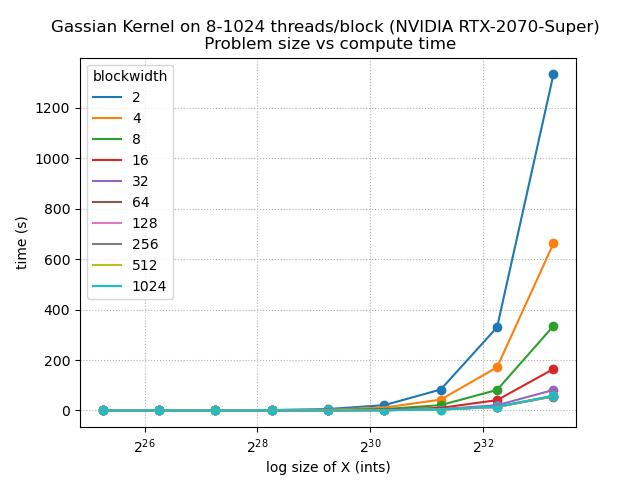
\includegraphics[width=0.8\textwidth]{"./experiment.jpg"}
  \caption{Problem size vs Compute time}
\end{figure}

\begin{table}[h!]
    \centering
    % Use csvsimple to load and display the CSV file
        \resizebox{\textwidth}{!}{%
        \csvautotabular{outfile.csv}  % Replace 'yourfile.csv' with your actual CSV file
    }
\end{table}


\subsection{Blockwidth vs Speedup}

\begin{figure}[H]
  \centering
  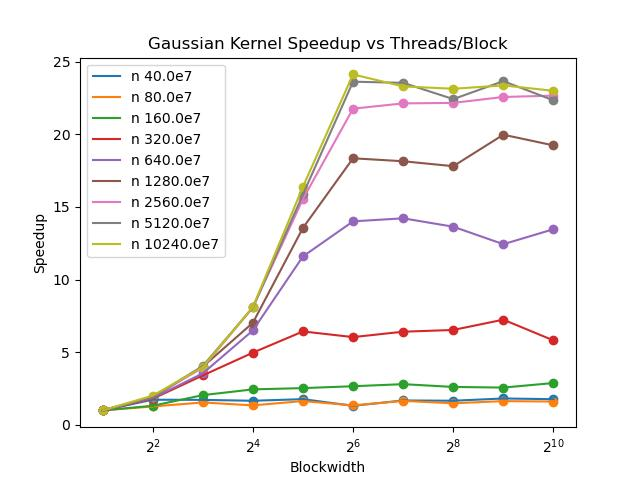
\includegraphics[width=0.8\textwidth]{"./speedup.jpg"}
  \caption{Blockwidth vs Speedup}
\end{figure}

\begin{table}[h!]
    \centering
    % Use csvsimple to load and display the CSV file
        \resizebox{\textwidth}{!}{%
        \csvautotabular{sp_outfile.csv}  % Replace 'yourfile.csv' with your actual CSV file
    }
\end{table}

\subsection{Blockwidth vs Efficiency}

\begin{figure}[H]
  \centering
  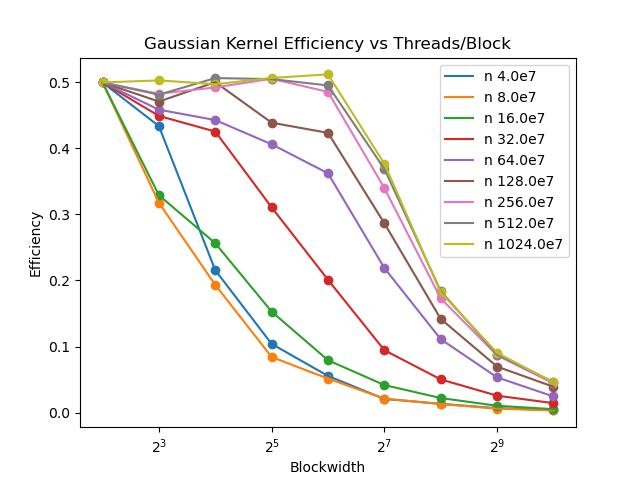
\includegraphics[width=0.8\textwidth]{"./efficiency.jpg"}
  \caption{Blockwidth vs Efficiency}
\end{figure}

\begin{table}[h!]
    \centering
    % Use csvsimple to load and display the CSV file
        \resizebox{\textwidth}{!}{%
        \csvautotabular{ep_outfile.csv}  % Replace 'yourfile.csv' with your actual CSV file
    }
\end{table}

\section{Discussion}
In Figure 1, We can observe the quadratic nature of the algorithm as the problem size increases. Initially as the blockwidth increases we are observing super-linear speedup. Its speeding up as fast as the problem size is increasing. This most likely means that the SM's are able to handle the blocksize quadratically increasing in size up until we hit 64 threads per block. It totally levels off in performance increase after this point. My assumption was that the device had allocated the maximum number of concurrently running blocks while the actual grid size was much larger causing the registers to be exhausted.

We can see this abrupt limitation in performance gains in Figure 2. Where we see the speedup is scaling with the increase in the problem size until we hit > 64 blockwidth. We are at least doubleing the speedup as the input size double which is a good sign but we can only achieve a max speedup of about 25 on 64 blockwidth. These speedup results are not great and suffer from inefficient parallelization methods (spawning n threads). Aside from the speedup limitation the quadratic speedup on a constant size input implies that the algorithm posesses strong scaling capabilities.

This can be seen in Figure 3. Where the max observed efficiency is about 50\%. This is conidered to not be efficient on the device and could be improved by different parallelization techniques such as limiting the number of running threads and utilizing shared memory on the device. Even though the maximum efficiency is 50\% The figure shows that efficiency is holding the same up until 128 blockwidth where it drops off but this is a sign of strong scaling.

\section{Conclusion}
Overall the algorithm will get the job done but it is by no means efficient or scalable past a certain hardware defined threshold. It possesses some strong scaling behaviors but is ultimately limited by the way it allocates the work to n threads which can exceed the devices limit of concurrent threads and register allocation. 

I did try to implement a different version of the algorithm I believe would have been able to deal with the observed limitation but wasn't able to finish it for sumbmission. The idea was to split the work load into a 2D grid where each block has a WxH that add up to the threadsPerBlock. Each thread would calculate multiple items for a given input that would balance the number of threads and keep it from dramatically increasing. The partial sums for each x was calculated along the y axis. Then the would be reduced within the block and stored in global memory. Another kernel would then take the results from all the blocks and perform a global reduction sum into y. I was limited by how much data I could store into shared memory and didn't want to allocate so much global memory on the device. 

\end{document}
